% TEXINPUTS=.:/home/hei2/Documents/LaTeX/myTexStyles:
% created for Journal of Heuristics 
% Time-stamp: "2011-07-18 14:17 hei2"
% if all fonts computer modern use -G1
% dvips -Ppdf -G0 <filename>
% http://www.springer.de/comp/lncs/authors.html

%!TEX TS-program = xelatex
%!TEX encoding = UTF-8 Unicode

%! xelatex joh.tex

\RequirePackage{fix-cm} 

\documentclass[smallextended]{svjour3} 
\smartqed  % flush right qed marks, e.g., at end of proof

\makeatletter
%\def\cl@chapter{\cl@chapter \@elt {theorem}}%bug in class
\def\cl@chapter{\@elt {theorem}}
\makeatother

\usepackage{mathptmx} % use Times fonts if available on your TeX system

\journalname{Journal of Heuristics}

\title{Learning Linear Composite Dispatch Rules for Scheduling}
\subtitle{Case study for the job-shop problem}

\author{Helga Ingimundardottir \and Thomas Philip Runarsson }
%\authorrunning{Short form of author list} % if too long for running head

\institute{H. Ingimundardottir \at
	Dunhaga 5, IS-107 Reykjavik, Iceland \\
	Tel.: +354-525-4704\\
	Fax: +354-525-4632\\
	\email{hei2@hi.is}\\
	\and
	T.P. Runarsson \at
	Hjardarhagi 2-6, IS-107 Reykjavik, Iceland \\
	Tel.: +354-525-4733\\
	Fax: +354-525-4632\\
	\email{tpr@hi.is}\\
}
\date{Received: \today / Accepted: date}
% The correct dates will be entered by the editor

\usepackage[english]{babel} 

% please place your own definitions here and don't use \def but
% \newcommand{}{}
\usepackage{url}

\usepackage{amssymb,bm,amsmath}
\newcommand{\vphi}{\bm{\phi}}
\newcommand{\vsigma}{\bm \sigma}
\newcommand{\vchi}{\bm \chi}
\newcommand{\R}{{\mathbb R}}

\newcommand{\inner}[2]{\big<{#1}\cdot{#2}\big>}
\newcommand{\abs}[1]{\lvert#1\rvert}
\newcommand{\norm}[1]{\lVert#1\rVert}
\newcommand{\argmax}{\mathop{\rm argmax}}
\newcommand{\nchoosek}[2]{\tiny \left(\begin{array}{c}#1\\#2\end{array}\right)}
\newcommand{\condset}[2]{\left\{#1\;\middle|\;#2\right\}}

% percentage relative deviation from optimality
\newcommand{\Namerho}{Deviation from optimality, $\rho$}
\newcommand{\namerho}{deviation from optimality, $\rho$}
\newcommand{\fullnamerho}{\namerho, defined by~\cref{eq:rho}}
\newcommand{\Problem}[2][ ]{$\mathcal{P}_{#2}^{#1}$}
\newcommand{\jrnd}[2]{\Problem[#1 \times #2]{j.rnd}}
\newcommand{\jrndJ}[2]{\Problem[#1 \times #2]{j.rnd,J_1}}
\newcommand{\jrndM}[2]{\Problem[#1 \times #2]{j.rnd,M_1}}
\newcommand{\jrndn}[2]{\Problem[#1 \times #2]{j.rndn}}
\newcommand{\frnd}[2]{\Problem[#1 \times #2]{f.rnd}}
\newcommand{\frndn}[2]{\Problem[#1 \times #2]{f.rndn}}
\newcommand{\fjc}[2]{\Problem[#1 \times #2]{f.jc}}
\newcommand{\fmc}[2]{\Problem[#1 \times #2]{f.mc}}
\newcommand{\fmxc}[2]{\Problem[#1 \times #2]{f.mxc}}
\newcommand{\dr}{dispatching rule}
\newcommand{\cdr}{composite priority \dr}
\newcommand{\sdr}{single priority \dr}
\newcommand{\Fsp}{Flow-shop}
\newcommand{\Jsp}{Job-shop}
\newcommand{\fsp}{flow-shop}
\newcommand{\jsp}{job-shop}
\newcommand{\FSP}{FSP}
\newcommand{\JSP}{JSP}
\newcommand{\Jrnd}{\JSP~random}
\newcommand{\JrndJ}{\JSP~random with job variation}
\newcommand{\JrndM}{\JSP~random with machine variation}
\newcommand{\Jrndn}{\JSP~random-narrow}
\newcommand{\Frnd}{\FSP~random}
\newcommand{\Frndn}{\FSP~random narrow}
\newcommand{\Fjc}{\FSP~job-correlated}
\newcommand{\Fmc}{\FSP~machine-correlated}
\newcommand{\Fmxc}{\FSP~mixed-correlated}

\newcounter{FeatCounter}
% job-related
\newcommand{\phiproc}{$\phi_1$}
\newcommand{\phistartTime}{$\phi_2$}
\newcommand{\phiendTime}{$\phi_3$}
\newcommand{\phiarrivalTime}{$\phi_4$}
\newcommand{\phitotalProc}{$\phi_5$}
\newcommand{\phiwait}{$\phi_6$}
\newcommand{\phiwrmJob}{$\phi_7$}
\newcommand{\phijobOps}{$\phi_8$}
\newcommand{\phiJobRelated}{\phiproc\!-\phijobOps}
% mac-related
\newcommand{\phimacFree}{$\phi_{9}$}
\newcommand{\phiwrmMac}{$\phi_{10}$}
\newcommand{\phimacOps}{$\phi_{11}$}
\newcommand{\phiMacRelated}{\phimacFree\!-\phimacOps}
% flow-related
\newcommand{\phislotsReduced}{$\phi_{12}$} 
\newcommand{\phislots}{$\phi_{13}$}
\newcommand{\phislotsTotal}{$\phi_{14}$} 
\newcommand{\phiFlowRelated}{\phislotsReduced\!-\phislotsTotal}
% schedule related
\newcommand{\phimakespan}{$\phi_{15}$}
\newcommand{\phiScheduleRelated}{\phimakespan}
% global
\newcommand{\phiSPT}{$\phi_{16}$}
\newcommand{\phiLPT}{$\phi_{17}$}
\newcommand{\phiLWR}{$\phi_{18}$}
\newcommand{\phiMWR}{$\phi_{19}$}
\newcommand{\phiRND}{$\phi_{20}$}
\newcommand{\phiSDRRelated}{\phiSPT\!-\phiMWR}
\newcommand{\phiGlobalRelated}{\phiMWR\!-\phiRND}
\newcommand{\phiLocalRelated}{\phiproc\!-\phimakespan}
\newcommand{\NrFeatLocal}{15}
\newcommand{\NrFeatGlobal}{5}
\newcommand{\NrFeatTotal}{20}

\hyphenation{heur-ist-ics}
\hyphenation{algo-rithm}

\usepackage{multirow}
\usepackage{rotating}
\newcommand{\rot}[1]{\begin{sideways}#1\end{sideways}}

\usepackage{paralist}

\usepackage{booktabs} % \toprule \midrule \bottomrule

\usepackage[colorinlistoftodos, textwidth=\marginparwidth]{todonotes}
\usepackage{comment}

\usepackage[capitalise,nameinlink]{cleveref} % must come last! % put your own shorthand declarations in this document

\begin{document}
\maketitle

\selectlanguage{english}

\begin{abstract}
\todo[inline]{Needs a rewrite}
Instead of creating new \dr s in an ad-hoc manner,
this study gives a framework on how to analyse heuristics for scheduling 
problems.  Before starting to create new \cdr s, 
meticulous research on optimal schedules can give an abundance of valuable 
information that can be utilised for learning new models.  For instance, it's 
possible to seek out when the scheduling process is most susceptible to 
failure.  Furthermore, the stepwise optimality of individual features imply 
their explanatory predictability. From which, a preference set is collected and 
a preference based learning model is created based on what feature states are 
preferable to others w.r.t. the end result, here minimising the final makespan.
By doing so it's possible to learn new \cdr s that 
outperform the models they are based on. 
Even though this study is based around the \jsp\ scheduling problem, it can be 
generalised to any kind of combinatorial problem.
\keywords{Scheduling \and Composite \dr s \and Machine Learning 
\and Feature Selection}
\end{abstract}

\section{Introduction}\label{sec:introduction}
The problem is to learn new problem specific priority \dr s for scheduling. 
A subclass of scheduling problems is the \jsp\ scheduling problem (JSP), 
which is widely studied in operations research.  \JSP\ deals with the 
allocation of tasks of competing resources where its goal is to optimise a 
single or multiple objectives.  Its analogy is from manufacturing industry 
where a set of jobs are broken down into tasks that must be processed on 
several machines in a workshop.  
Furthermore, its formulation can be applied on a wide variety of practical 
problems in real-life applications which involve decision making, therefore its
problem-solving capabilities has a high impact on many manufacturing 
organisations.

Generally, \jsp\ is solved by applying a hand-crafted dispatching rule (DR) for 
a given problem space. 
Due to the exorbitant amounts of DRs to choose from, and any kind of alteration 
to the problem space, this can become quite a time-consuming selection process 
for the heuristic designer, which any kind of automation would alleviate 
immensely. 
% automation for selecting DRs #1 - Portfolio
With meta heuristics one can use existing DRs, and use for example 
portfolio-based algorithm selection \cite{Rice76,Gomes01}, either based on a 
single instance or class of instances \cite{Xu07} to determine which DR to 
choose from. 
% automation for selecting DRs #2 - ACO
Implementing ant colony optimisation to select the best DR 
from a selection of nine DRs for \JSP, experiments from \cite{Korytkowski13} 
showed that the choice of DR do affect the results and that for all performance 
measures considered. They showed that it was better to have a all the DRs to 
choose from rather than just a single DR at a time.

Heuristics algorithms for scheduling are typically either a construction or 
improvement heuristics. The improvement heuristic starts with a complete 
schedule and then tries to find similar, but better schedules.  A construction 
heuristic starts with an empty schedule and adds one job at a time until the 
schedule is complete. The work presented here will focus on construction 
heuristics, \dr s, although the techniques developed could be adapted to 
improvement heuristics also. 

\todo[inline,color=pink]{Direct search (GA based, Poli, etc)}

Genetic algorithms (GA) are one of the most widely used approaches in \JSP\ 
literature \cite{Pinedo08}. However, in that case an extensive number of 
schedules need to be evaluated, and even for low dimensional \JSP\ that can 
quickly become computationally infeasible.
GAs can be used directly on schedules 
\cite{Cheng96,Cheng99,Tsai07,Qing-dao-er-ji12,Ak12,Meeran12}, however, in that 
case there are many concerns that need to be dealt with. To begin with there 
are nine encoding schemes for representing the schedules \cite{Cheng96}, in 
addition there has to be special care when applying cross-over and mutation 
operators in order for the schedules, now in the role of `chromosomes,' to 
still remain feasible. 

Another approach is to apply GAs indirectly to \JSP , via dispatching rules, 
i.e., Dispatching Rules Based Genetic Algorithms (DRGA) 
\cite{Vazquez-Rodriguez09,Dhingra10,Nguyen13} where a solution is no longer a 
\emph{proper} schedule but a \emph{representation} of a schedule via applying 
certain dispatching rules consecutively. 
DRGA are a special case of \emph{genetic programming} \cite{Koza05} which is 
the most predominant approach in hyper-heuristics is a framework of creating 
\emph{new} heuristics from a set of  predefined heuristics via GA optimisation 
\cite{Burke10}. 

A prevalent approach to solving \JSP\ is to combine several relatively \sdr s 
such that they may benefit each other for a given problem space. 
% automation for selecting DRs #3 - GA
The approach in \cite{InRu14}, was to automate that selection, by 
translating dispatching rules into measurable features and optimising what 
their contribution should be via evolutionary search. The framework is straight 
forward and easy to implement and showed promising and robust results, 
as models were trained on a lower dimension, and validated on higher dimension. 
Moreover, \cite{InRu14} showed that the choice of objective 
function  for evolutionary search is worth investigating. Since the 
optimisation is based on minimising the expected mean of the fitness function 
over a large set of problem instances, which can vary within. Then normalising 
the objective function can stabilise the optimisation process away from local 
minima. 

% automation for selecting DRs #4 - GA
By applying genetic programming (GP) on a terminal set of job attributes for 
flexible \jsp,\footnote{Flexible \jsp\ allows jobs to be processed on different 
machines, i.e., the problem has the additional complexity of making a routing 
decision of operations to machines.} \cite{Tay08} optimised a multi-objective 
\jsp~(transformed into a single objective by linearly combining their 
objectives) with promising results 
compared to the benchmarks DRs from the literature.
The main drawback, is that the rules from their GP framework is quite complex, 
and difficult to contrive a meaningful description to a layman.
In fact, \cite{Hildebrandt2010} revisited the experiments from \cite{Tay08} for 
dynamic \jsp,\footnote{\Jsp\ is considered dynamic when the processing times 
are not known prior to their arrival.} and tested it against some \sdr s, and 
found that it only slightly outperformed ERD, and was beat by SPT. The reason 
behind this staggering change in performance, is most likely due to the choice 
of objective function, and the underlying problem spaces that were used in 
training. It's argued that the randomly generated problem instances aren't a 
proper representative for real-world long-term \jsp\ applications, e.g., by the 
narrow choice of release times, yielding schedules that are overloading in the 
beginning phases.

A novel iterative \dr s that were evolved with GP for \JSP, \cite{Nguyen13} 
learned from completed schedules in order to iteratively improve new ones. 
At each dispatching step, the method can utilise the current feature space to 
\emph{correctify} some possible \emph{bad} dispatch made previously (sort of 
reverse lookahead). Their method is straightforward, and thus easy to 
implement and more importantly computationally inexpensive, although the 
authors do stress that there is still remains room for improvement.

Adopting a two-stage hyper-heuristic approach to generate a set of 
machine-specific DRs for dynamic \jsp, \cite{Pickardt2013} used GP to evolve 
CDRs from basic attributes, along with evolutionary algorithm to assign a CDR 
to a specific machine. 
The problem space consists of \jsp s in semiconductor manufacturing, with 
additional shop constraints, as machines are grouped to similar work centres, 
which can have different set-up time, workload, etc. 
In fact, the GP emphasised on efficiently dispatching on the work 
centres with set-up requirements and batching capabilities, which are rules 
that are non-trivial to determine manually.

In the field of Artificial Intelligence, \cite{Meeran12} point out that despite 
their `intelligent' solutions, the effectiveness of finding the optimum has 
been rather limited. This is the general case for GAs, as they are not well 
suited for fine-tuning around the optimum \cite{Cheng99}. 
However, combined with local-search methodologies, they can be improved upon 
significantly, as \cite{Meeran12} showed with the use of a hybrid method using 
Genetic Algorithms (GA) and Tabu Search (TS). 
Therefore, getting the best of both worlds, namely, the diverse global search 
obtained from GA and being complemented with the intensified local search 
capabilities of TS. 
Now, hybridisation of global and local methodologies is non-trivial. In 
general combination of the two improves performance, however, they often come 
at a great computational cost.  

\todo[inline,color=green]{Another citation from Poli, besides \cite{Koza05}?}

\todo[inline,color=pink]{Reinforcement learning based, Diettrich, also Kendall 
\& Burke}

Using improvement heuristics, \cite{Zhang95} studied space shuttle payload 
processing by using reinforcement learning (RL), in particular, temporal 
difference learning. 
Starting with a relaxed problem, each job was scheduled as early as its 
temporal partial order would permit, there by initially ignoring any resource 
constraints on the machines, yielding the schedule's critical path. Then the 
schedule would be repaired so the resource constraints were satisfied in the 
minimum amount of iterations.

Meta learning can be very fruitful in RL, as experiments from 
\cite{Kalyanakrishnan11} discovered some key discriminants between 
competing algorithms for their particular problem instances, which provided 
them with a hybrid algorithm which combines the strengths of the algorithms.

\todo[inline,color=green]{Burke \cite{Burke06} on reinforcement learning from 
2006. However, \cite{Burke10} from 2010 above (GA section)}

Using case based reasoning for timetable scheduling, training data in 
\cite{Burke06} is guided by the two best heuristics in the literature.
They point out that in order for their framework to be successful, problem 
features need to be sufficiently explanatory and training data need to be 
selected carefully so they can suggest the appropriate solution for a specific 
range of new cases. Stressing the importance of meaningful feature selection. 

\todo[inline,color=pink]{Supervised learning (Siggi, etc)}

A recent editorial of the state-of-the-art approaches in advanced \dr s for 
large-scale manufacturing systems by \cite{Chen13} points out that:
\lq\lq ... most traditional \dr s are based on historical data. 
With the emergence of data mining and on-line analytic processing, dispatching 
rules can now take predictive information into account.\rq\rq~The importance of 
automated discovery of DR was also emphasised by \cite{Monch13}. 
Several of successful implementations in the field of semiconductor wafer 
fabrication facilities are discussed, however, this sort of investigation is 
still in its infancy.

The alternative to hand-crafting heuristics, is to implement an automatic way 
of learning heuristics using a data driven approach. 
Data can be generated using a known heuristic, such an approach is taken in 
\cite{Siggi05} for single-machine \jsp\ %, namely $5\times1$, 
where a LPT-heuristic is applied.
Afterwards, a decision tree is used to create a \dr\ with similar logic. 
However, this method cannot outperform the original 
LPT-heuristic used to guide the search. 
This drawback is confronted in \cite{Malik08,Russell09,Siggi10} by using an 
optimal scheduler, computed off-line. 
The optimal solutions are used as training data and a decision tree 
learning algorithm applied as before. Preferring simple to complex models, the 
resulting \dr s gave significantly better schedules than using popular 
heuristics in that field, and a lower worst-case factor from optimality. 

The focus on this study is better understanding of \emph{how} and \emph{when} 
\dr s work in general, in order to mediate the set-up for the 
learning problem.
For this reason, we propose a framework for learning the indicators of optimal 
solutions, such as done by \cite{Siggi10}, as an in-depth analysis of a expert 
policy gives a benchmark of what is theoretically possible to learn. 

The study shows that during the scheduling process, it varies \emph{when} it's 
most fruitful to make the `right' decision, and depending on the problem space 
those pivotal moments can vary greatly. 

Although, using optimal trajectory for creating training data gives vital 
information on how to learn good scheduling rules, it is a good starting point, 
but not sufficient. This is due to the fact our models are only based on 
optimal decisions, then once we make a suboptimal choice we are in uncharted 
territory and its effects are relatively unknown. For this reason, it is of 
paramount importance to inspect the actual end-performance when choosing a 
suitable model, not just staring blindly at the validation accuracy. Moreover, 
different measures on how to report training accuracy is discussed.

\todo[inline,color=pink]{Outline of paper}
The outline of the paper is the following, \cref{sec:problemdef} gives the 
mathematical formalities of the scheduling problem, and  
\cref{sec:DR} describes the main attributes for \jsp, 
and goes into how to create schedules with \dr s. In \cref{sec:learnCDR} we 
show how to create \cdr s using preference learning, focusing on how to 
compare operations and collect training data.
\Cref{sec:opt} sets up the framework for learning from optimal schedules. In 
particular, the probability of choosing optimal decisions and the effects of 
making a suboptimal decision. 
Furthermore, the optimality of common \sdr s is investigated.
With those guidelines, \cref{ch:expr:CDR} goes into detail how to create 
meaningful \cdr s, with the importance of good feature 
selection and the polysemy of how to report accuracy. 
The paper finally concludes in \cref{sec:con} with discussion and conclusions.

%\setcounter{tocdepth}{2} \tableofcontents

\section{\Jsp~Scheduling}\label{sec:problemdef}
The \jsp~problem (\JSP) involves the scheduling of jobs on a set of 
machines. Each job consists of a number of operations which are then processed 
on the machines in a predetermined order. An optimal solution to the problem 
will depend on the specific objective. 
% For example, the optimal schedule may be the time needed to complete
% all jobs, i.e., the minimum makespan.

In this study we will consider the $n\times m$ \JSP, where $n$ jobs, 
$\mathcal{J}=\{J_j\}_{j=1}^n$, are scheduled on a finite set, 
$\mathcal{M}=\{M_a\}_{a=1}^m$, of $m$ machines. The index $j$ refers to a job 
$J_j\in\mathcal{J}$ while the index  $a$ refers to a machine 
$M_a\in\mathcal{M}$. 
If a job requires a number of processing steps or operations, then the pair 
$(j,a)$ refers to the operation, i.e., processing the task of job $J_j$ on 
machine $M_a$. 

Each job $J_j$ has an indivisible operation time (or cost) on machine $M_a$, 
$p_{ja}$, which is assumed to be integral and finite. 
Starting time of job $J_j$ on machine $M_a$ is denoted $x_s(j,a)$ and its 
end time is denoted $x_e(j,a)$ where, 
\begin{equation}  x_e(j,a):=x_s(j,a)+p_{ja} \end{equation} 
Each job $J_j$ has a specified processing order through the machines, it is a 
permutation vector, $\vsigma_j$, of $\{1,..,m\}$, representing a job $J_j$ can 
be processed on $M_{\vsigma_j(a)}$ only after it has been completely processed 
on $M_{\vsigma_j(a-1)}$, i.e.,
\begin{equation}\label{eq:permutation}
x_s(j,\vsigma_j(a)) \geq x_e(j,\vsigma_j(a-1)) 
\end{equation}
for all $J_j\in\mathcal{J}$ and $a\in\{2,..,m\}$. 
Note, that each job can have its own distinctive flow pattern through the 
machines, which is independent of the other jobs. 
However, in the case that all jobs share the same \emph{fixed} permutation 
route, referred to as \fsp~(\FSP). 
A commonly used subclass of \FSP\ in the literature is permutation \fsp, which 
has the added constraint that the processing order of the jobs on the machines 
must be identical as well, i.e., no passing of jobs allowed \cite{Stafford88}.

The disjunctive condition that each machine can handle at most one job at a 
time is the following,
\begin{equation}\label{eq:oneJobPerMac}
x_s(j,a) \geq x_e(j',a) \quad\textrm{or}\quad x_s(j',a) \geq x_e(j,a)  
\end{equation}
for all $J_j,J_{j'}\in\mathcal{J},\; J_j\neq J_{j'}$ and $M_a\in\mathcal{M}$. 

The objective function is to minimise its maximum completion times for all 
tasks, commonly referred to as the makespan, $C_{\max}$, which is defined as 
follows,
\begin{equation}
C_{\max} := 
\max\left\{x_e(j,\vsigma_j(m))\;\middle|\;J_j\in\mathcal{J}\right\}.\label{eq:makespan}
\end{equation} 
This family of scheduling problems is denoted by $J||C_{\max}$ 
\cite{Pinedo08}.
Additional constraints commonly considered are job release-dates and due-dates 
or sequence dependent set-up times, however, these will not be considered here. 

In order to find an optimal (or near optimal) solution for scheduling problems 
one could either use exact methods or heuristics methods. Exact methods 
guarantee an optimal solution. However, \jsp\ scheduling is strongly NP-hard 
\cite{Garey76:NPhard}. Any exact algorithm generally suffers from the curse of 
dimensionality, which impedes the application in finding the global optimum in 
a reasonable amount of time. 
Using a state-of-the-art software for solving scheduling problems, such as 
LiSA %\footnote{LiSA is distributed under the GNU General Public License, and 
%is available at \url{http://www.math.ovgu.de/Lisa.html}.} 
(A Library of Scheduling Algorithms) \cite{LiSA}, which includes a specialised 
version of branch and bound that manages to find optimums for \jsp\ problems of 
up to $14\times14$ \cite{Ru12}. However, problems that are of greater size, 
become intractable. 
Heuristics are generally more time efficient but 
do not necessarily attain the global optimum. Therefore, \jsp\ has the 
reputation of being notoriously difficult to solve. 
As a result, it's been widely studied in deterministic scheduling theory and 
its class of problems has been tested on a plethora of different solution 
methodologies from various research fields \cite{Meeran12}, all from simple and 
straight forward \dr s to highly sophisticated frameworks.


\section{Priority Dispatching Rules} \label{sec:DR}

Priority \dr s determine, from a list of incomplete jobs, 
$\mathcal{L}$, which job should be dispatched next. This process is illustrated 
in \Cref{fig:jssp:example}, where an example of 
a temporal partial schedule of six-jobs scheduled on five-machines is given. 
The numbers in the boxes represent the job identification $j$. 
The width of the box illustrates the processing times for a given job for a 
particular machine $M_a$ (on the vertical axis). 
The dashed boxes represent the resulting partial schedule for when a particular 
job is scheduled next. 
Moreover, the current $C_{\max}$ is denoted by a dotted vertical line. 
The object is to keep this value as small as possible once all operations are 
complete. As shown in the example there are $15$ operations already scheduled. 
The \textit{sequence} of dispatches used to create this partial schedule is,
\begin{equation}
	\vchi=\left(J_3,J_3,J_3,J_3,J_4,J_4,J_5,J_1,J_1,J_2,J_4,J_6,J_4,J_5,J_3\right)
\end{equation}
and refers to the sequential ordering of job dispatches to machines, i.e., $(j,a)$; 
the collective set of allocated jobs to machines is interpreted by its 
sequence, is referred to as a \emph{schedule}.
A \emph{scheduling policy} will pertain to the manner in which 
the sequence is determined from the available jobs to be scheduled. 
In our example the available jobs is given by the job-list
$\mathcal{L}^{(k)}=\{J_1,J_2,J_4,J_5,J_6\}$ with the five potential jobs 
to be dispatched at step $k=16$ (note that $J_3$ is completed).

Deciding which job to dispatch is, however, not sufficient, one must also know 
where to place it. In order to build tight schedules it is sensible to place a 
job as soon as it becomes available and such that the machine idle time is 
minimal, i.e., schedules are non-delay. 
There may also be a number of different options for such a placement. 
In \cref{fig:jssp:example} one observes that $J_2$, to be scheduled on $M_3$, 
could be placed immediately in a slot between $J_3$ and $J_4$, or after $J_4$ 
on this machine. 
If $J_6$ had been placed earlier, a slot would have been created between it and 
$J_4$, thus creating a third alternative, namely scheduling $J_2$ after $J_6$. 
The time in which machine $M_a$ is idle between consecutive jobs $J_j$ and 
$J_{j'}$ is called idle time, or slack, 
\begin{equation} 
s(a,j):=x_s(j,a)-x_e(j',a) \label{eq:slack}
\end{equation}
where $J_j$ is the immediate successor of $J_{j'}$ on $M_a$. 

Construction heuristics are designed in such a way that it limits the search 
space in a logical manner, respecting not to exclude the 
optimum\todo{Are you sure about this, I don't think this is 
right!}\todo[color=pink]{What do you mean? The slot placement matters, I did 
tests way back when. 
97\% vs. 100\% reproducability of achieving optimal solution.}. Here, the 
construction heuristic is to schedule the dispatches as closely together as 
possible, i.e., minimise the schedule's idle time. 
More specifically, once an operation $(j,a)$ has been chosen from the job-list, 
$\mathcal{L}$, by some dispatching rule, it can placed immediately after (but 
not prior) $x_e(j,\vsigma_j(a-1))$ on machine $M_a$ due to constraint 
\cref{eq:permutation}. 
However to guarantee that constraint \cref{eq:oneJobPerMac} is not violated, 
idle times $M_a$ are inspected, as they create flow time  which $J_j$ can 
occupy. Bearing in mind that $J_j$ release time is $x_e(j,\vsigma_j(a-1))$ one 
cannot implement \cref{eq:slack} directly, instead it has to be updated as 
follows,
\begin{equation}
\tilde{s}(a,j'):= x_s(j'',a)-\max\{x_e(j',a),x_e(j,\vsigma_j(a-1))\} % 
%\textrm{ if } x_e(j,\vsigma_j(a-1)\geq x_e(j',a) 
\end{equation}
for all already dispatched jobs $J_{j'},J_{j''}\in \mathcal{J}_a$ where 
$J_{j''}$ is $J_{j'}$ successor on $M_a$. Since pre-emption is not allowed, the 
only applicable slots are whose idle time can process the entire operation, 
i.e.,
\begin{equation}
\tilde{S}_{ja} := \condset{J_{j'}\in \mathcal{J}_a}{\tilde{s}(a,j')\geq p_{ja} 
}\label{eq:slots}.
\end{equation} 
The placement rule applied will decide where to place the job and 
is an intrinsic heuristic of the construction heuristic, chosen independently 
of the priority dispatching rule applied. 
Different placement rules could be considered for selecting a slot from 
\cref{eq:slots}, e.g., if the main concern were to utilise the slot space, then 
choosing the slot with the smallest idle time would yield a closer-fitted 
schedule and leaving greater idle times undiminished for subsequent dispatches 
on $M_a$.
In our experiments cases were discovered where such a placement can rule out 
the possibility of constructing optimal solutions.
This problem, however, did not occur when jobs are simply placed as early as 
possible, which is beneficial for subsequent dispatches for $J_j$. 
For this reason it will be the placement rule applied here.

\begin{figure}[t!]\centering
	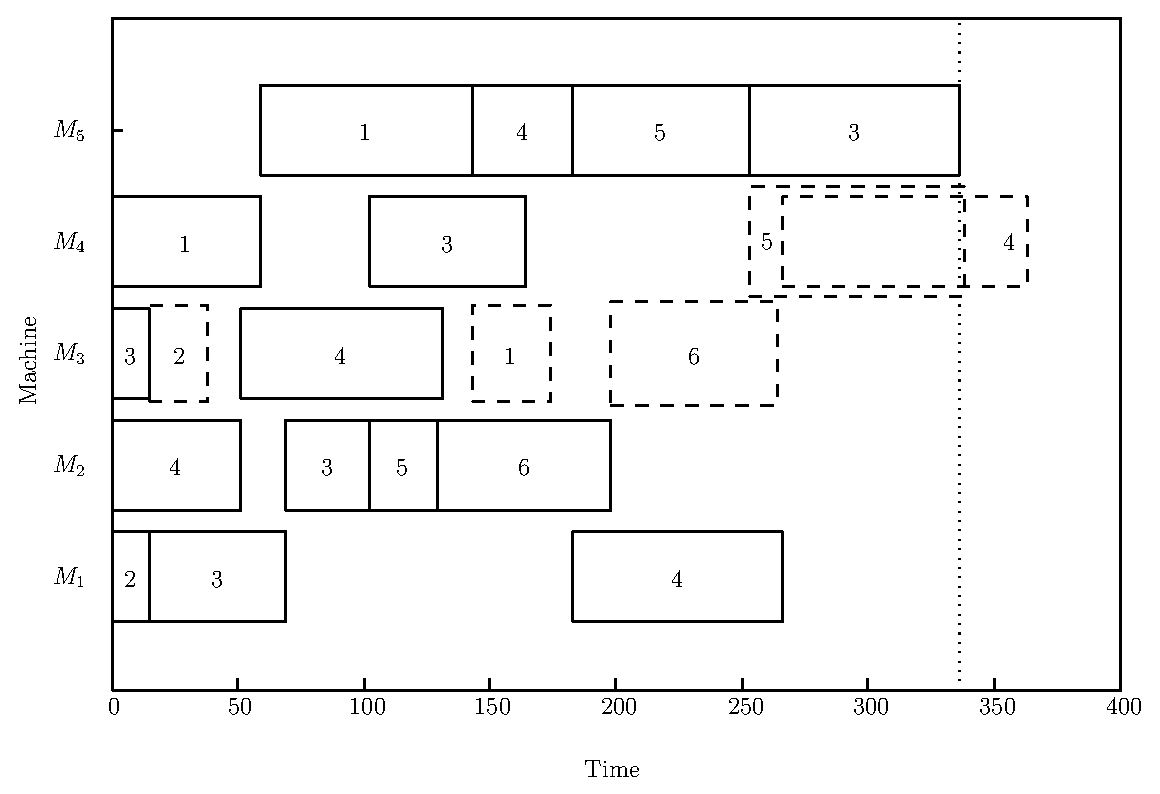
\includegraphics[width=0.8\textwidth]{figures/jssp_example_nocolor}
	\caption[Gantt chart of a partial \JSP\ schedule]{Gantt chart of a
		partial \JSP\ schedule after 15 dispatches: Solid and dashed boxes
		represent $\vchi$ and $\mathcal{L}^{(16)}$, respectively. Current
		$C_{\max}$ denoted as dotted line.}
	\label{fig:jssp:example}
\end{figure}

%\subsection{Priority Dispatching Rules}\label{ch:dispatchrules}
% \subsection{Simple priority \dr s}
%Dispatching rules are of a construction heuristics, where one starts with an 
%empty schedule and adds sequentially on %one operation (or tasks) at a time. 

Priority \dr s will use attributes of operations, such as processing time, 
in order to determine the job with the highest priority. \todo{Inconsist: 
\emph{attribute} versus \emph{feature}}\todo{Let us use attribute rather ad features, search and replace entire document!}
Consider again \Cref{fig:jssp:example}, if the job with the shortest processing 
time (SPT) were to be scheduled next, then $J_2$ would be dispatched. 
Similarly, for the longest processing time (LPT) heuristic, $J_5$ would have the highest priority. 
Dispatching can also be based on attributes related to the partial schedule. 
Examples of these are dispatching the job with the most work remaining (MWR) or 
alternatively the least work remaining (LWR). A survey of more than $100$ of 
such rules are presented in \cite{Panwalkar77}. 
However, the reader is referred to an in-depth survey for simple or 
\emph{\sdr} (SDR) by \cite{Haupt89}.  
The SDRs assign an index to each job in the job-list and is generally only 
based on a few attributes and simple mathematical operations.

\begin{table}[t!] \centering
	\caption[Attribute space $\mathcal{A}$ for \JSP]{Attribute space 
	$\mathcal{A}$ for \JSP\ where job $J_j$ on machine $M_a$ given the 
	resulting temporal schedule after operation $(j,a)$.
	}
	\label{tbl:jssp:feat}
	\centering
\renewcommand{\arraystretch}{1.5}
\begin{tabular}{clll} %p{0.45\textwidth}|p{0.4\textwidth}|}
	\toprule
	$\vphi$          & Feature description                       & Mathematical formulation                                                           & Shorthand    \\ 
	%\hline  \multicolumn{4}{c}{\textbf{Local features}}  \\
	\midrule
	\multicolumn{4}{c}{\textbf{job related}}\\
	\phiproc         & job processing time                       & $p_{ja}$                                                                           & proc         \\
	\phistartTime    & job start-time                            & $x_s(j,a)$                                                                         & startTime    \\
	\phiendTime      & job end-time                              & 
	$x_e(j,a)$                                                                    
	     &
	 endTime      \\
	\phiarrivalTime  & job arrival time                          & 
	$x_e(j,a-1)$                                                                  
	     &
	 arrival      \\ 
	\phitotalProc    & total processing time                     & $\sum_{a\in \mathcal{M}}p_{ja}$                                                    & totalProc    \\
	\phiwait         & time job had to wait                      & 
	$x_s(j,a)-x_e(j,a-1) 
	$                                                             & wait         
	\\   
	\phiwrmJob       & total work remaining for job              & $\sum_{a'\in\mathcal{M}\setminus \mathcal{M}_{j}}p_{ja'}$                          & wrmJob       \\
	\phijobOps       & number of assigned operations for job     & $|\mathcal{M}_j|$                                                                  & jobOps       \\ 
	\midrule
	\multicolumn{4}{c}{\textbf{machine related}}\\
	\phimacFree      & when machine is next free                 & $\max_{j'\in 
	\mathcal{J}_a} \{x_e(j',a)\}$                                         & 
	macFree      \\
	\phiwrmMac       & total work remaining for machine          & $\sum_{j'\in\mathcal{J}\setminus \mathcal{J}_{a}}p_{j'a} $                         & wrmMac       \\
	\phimacOps       & number of assigned operations for machine & $|\mathcal{J}_a|$                                                                  & macOps       \\
	\phislotsReduced & change in idle time by assignment         & $\Delta 
	s(a,j)$                                                                    & 
	reducedSlack \\
	\phislots        & total idle time for machine               & $\sum_{j'\in 
	\mathcal{J}_a}s(a,j')$                                                & 
	slack        \\
	\phislotsTotal   & total idle time for all machines          & $\sum_{a'\in 
	\mathcal{M}}\sum_{j'\in \mathcal{J}_{a'}}s(a',j')$                    & 
	totalSlack   \\
	\phimakespan     & current makespan                          & 
	$\max_{(j',a')\in \mathcal{J} \times 
	\mathcal{M}_{j'}}\{x_f(j',a')\}$              & makespan     \\
	\bottomrule
\end{tabular}


\end{table}

Designing priority \dr s requires recognizing the important 
attributes of the partial schedules needed to create a good scheduling rule. 
These attributes attempt to grasp key features of the schedule being 
constructed. Which attributes are most important will necessarily depend on the
objectives of the scheduling problem. 
Attributes used in this study applied for 
each possible operation are given in \cref{tbl:jssp:feat}, where the set of 
machines already dispatched for $J_j$ is $\mathcal{M}_j\subset\mathcal{M}$, 
and similarly, $M_a$ has already had the jobs $\mathcal{J}_a\subset\mathcal{J}$ 
previously dispatched.
The attributes of particular interest were obtained by inspecting the 
aforementioned SDRs. Attributes \phiJobRelated\ and \phiMacRelated\ are 
job-related and machine-related, respectively.
In fact, \cite{Pickardt2013} note that in the current literature, there is a 
lack of global perspective in the attribute space, as omitting them won't 
address the possible negative impact an operation $(j,a)$ might have on other 
machines at a later time, it is for that reason we consider attributes such as 
\phiSlackRelated, that are slack related and are a means of indicating the 
current quality of the schedule.
All of attributes, $\vphi$, vary throughout the scheduling process, 
w.r.t. operation belonging to the same time step $k$, with the exception of 
\phijobTotProcTime\ and \phimacTotProcTime\ which are static for a given 
problem instance but varying for each $J_j\in\mathcal{J}$ and 
$M_a\in\mathcal{M}$, respectively. 

Priority \dr s are attractive since they are relatively easy to 
implement, 
fast and find good schedules. In addition, they are relatively easy to 
interpret, which makes them desirable for the end-user.
However, they can also fail unpredictably. 
A careful combination of \dr s have been shown to perform significantly better 
\cite{Jayamohan04}. These are referred to as \emph{\cdr s} 
(CDR), where the priority ranking is an expression of several \sdr s. 
CDRs deal with a greater number of more complicated features constructed from the schedules attributes. In short a CDR is a combination of several SDRs. For 
instance let $\pi$ be a CDR comprised of $d$ DRs, then 
the index $I$ for $J_j\in\mathcal{L}^{(k)}$ using $\pi$ is, 
\begin{equation}
	I_j^{\pi} = \sum_{i=1}^d w_i \cdot \pi_i(\vphi_j) \label{eq:CDR}
\end{equation}
where $w_i>0$ and $\sum_{i=0}^d w_i = 1$ with $w_i$ giving the weight of the 
influence of $\pi_i$ (which could be a SDR or another CDR) to $\pi$. Note, 
each $\pi_i$ is function of $J_j$'s attributes $\vphi_j$.  
At each time step $k$, an operation is dispatched which has the highest 
priority.  If there is a 
tie, some other priority measure is used. Generally the priority dispatching 
rules are static during the entire scheduling process, however, ties could also 
be broken randomly (RND). 

Investigating 11 SDRs for JSP, \cite{Lu13} created a pool of 33 CDRs that 
strongly outperformed the ones they were based on, by using multi-contextual 
functions based on either on job waiting time or machine idle time 
(similar to \phiwait\ and \phimacSlack\ in \cref{tbl:jssp:feat}), i.e., the 
CDRs are a combination of those two key attributes and then the SDRs. 
However, there are no combinations of the basic SDRs explored, only those two 
attributes.  
Similarly, using priority rules to combine 12 existing DRs from the literature, 
\cite{Yu13} had 48 CDR combinations, yielding 48 different models 
to implement and test. 
It is intuitive to get a boost in performance by introducing new CDRs, since 
where one DR might be failing, another could be excelling so combining them 
together should yield a better CDR. However, these approaches introduce fairly 
ad-hoc solutions and there is no guarantee the optimal combination of 
\dr s are found.


The \cdr\ presented in \cref{eq:CDR} can be 
considered as a special case of a the following general linear value function,
\begin{equation}\label{eq:jssp:linweights}
	h(\vchi)=\sum_{i=1}^d w_i\phi_i(\vchi).
\end{equation}
when $\phi_i=\pi_i(\vec{\phi})$ and the job to be dispatched, $J_{j^*}$, corresponds to the one highest 
value, i.e.,
\begin{equation}\label{eq:lin}
	J_{j^*}=\argmax_{J_j\in \mathcal{L}}\; h(\vphi_j)
\end{equation}
Similarly, \sdr s may be described by this linear model. For instance, let all 
$w_i=0$, but with following exceptions: $w_1=-1$ for SPT, $w_1=+1$ for LPT, 
$w_7=-1$ for LWR and $w_7=+1$ for MWR. Generally the weights $\vec{w}$ are 
chosen by the designer or the 
rule apriori.  A more attractive approach would be to learn these weights from 
problem examples directly. We will now investigate how this may be accomplished.

\section{Performance Analysis of Priority Dispatching Rules}\label{sec:learnCDR}

In this section we will describe concerns that must be addressed when learning 
new priority \dr s. At the same time we will describe the experimental setup 
used in our study. The matters that must be addressed are as 
follows
\begin{enumerate*}[itemjoin*={{, and finally }}]
\item the problem instances used for learning and their optimal solutions
\item the reconstruction of the optimal solution using a \dr
\item the construction of the training set used for learning
\item the machine learning procedure used must be decided
\end{enumerate*}

\subsection{Problem Instances}\label{sec:data:sim}

The class of problem instances used in our studies is the \jsp\ scheduling 
problem described in section~\ref{sec:problemdef}. Each instance will have 
different processing times, machine ordering and dimensions. Each instance will 
therefore create different challenges for a priority dispatching rule. 
Dispatching rules learned will be customized for the problems used for their 
training. For real world application using historical data would be most 
appropriate. The aim would be to learn a dispatching rule that works well on 
average for a distribution of problem instances. To illustrate the performance 
difference of priority \dr s on different problem distributions, 
within the same class of problems, consider the following three cases.
Problem instances for JSP are generated stochastically by fixing the number of 
jobs and machines to ten. A discrete processing time is sampled independently 
from a discrete uniform distribution from the interval $I=[u_1,u_2]$, i.e., 
$\vec{p}\sim \mathcal{U}(u_1,u_2)$. 
The machine order is a random permutation of all of the machines in the 
\jsp\. Two different processing times distributions were explored, namely 
\jrnd{n}{m}  
where $I=[1,99]$ and \jrndn{n}{m} where $I=[45,55]$. These instances 
are referred to as random and random-narrow, respectively. In addition we 
consider 
the case where the machine order is fixed and the same for all jobs, i.e. 
$\vec{\sigma}=\{1,\ldots,m\}$
where $\vec{p}\sim\mathcal{U}(1,99)$. These jobs are denoted by \frnd{n}{m} and 
is analogous to 
\jrnd{n}{m}.

The goal is to minimize the makespan, $C_{\max}$. The optimum 
makespan is denoted $C_{\max}^{\text{opt}}$, and the makespan obtained from the 
scheduling policy $A$ under inspection by $C_{\max}^{A}$. Since the optimal 
makespan varies between problem instances the performance measure is the 
following,
\begin{equation}\label{eq:ratio}
\rho=\frac{C_{\max}^{A}-C_{\max}^{\text{opt}}}{C_{\max}^{\text{opt}}}\cdot
100\%
\end{equation}
which indicates the percentage relative deviation from optimality. 
\Cref{fig:boxplot:SDR} depicts the box-plot for \cref{eq:ratio} when using the 
SDRs from \cref{sec:DR} for all of the problem spaces from \cref{tbl:data:sim}.

\begin{table}\centering
  \caption[Problem space distributions used in experimental studies.]{Problem 
    space distributions used in experimental studies. Note, problem instances 
    are synthetic and each problem space is i.i.d. 
  }\label{tbl:data:sim}
  {\renewcommand{\arraystretch}{1.5}
	\begin{tabular}{clcccl}\toprule 
		type & name & size ($n\times m$) & $N_{\text{train}}$ & 
		$N_{\text{test}}$ & note
		\\ \midrule
		\multirow{2}{*}{{JSP}}
		%&\jrnd{8}{8} &$8\times8$& -- & 500 & random \\
		  & \jrnd{10}{10}  & $10\times10$ & 300 & 200 & random        \\
		%&\jrnd{12}{12} &$12\times12$& -- & 500 & random \\
		%&\jrndn{8}{8} &$8\times8$& -- & 500 & random-narrow \\ 
		  & \jrndn{10}{10} & $10\times10$ & 300 & 200 & random-narrow \\ 
		%&\jrndn{12}{12} &$12\times12$& -- & 500 & random-narrow \\ 
		\midrule
		\multirow{1}{*}{{FSP}}
		%&\frnd{8}{8} &$8\times8$& --&500& random \\ 
		  & \frnd{10}{10}  & $10\times10$ & 300 & 200 & random        \\ 
		%&\frnd{12}{12} &$12\times12$& --&500& random \\ 
		\bottomrule
	\end{tabular}
}
\end{table} 

\begin{figure}
  \centering
  \includegraphics[width=1\linewidth]{figures/{boxplotRho_SDR_10x10}.pdf}
  \caption{Box-plot for deviation from optimality, $\rho$, (\%) for SDRs}
  \label{fig:boxplot:SDR}
\end{figure}

\subsection{Reconstructing optimal solutions}\label{sec:opt:sdr}

When building a complete schedule, $\ell=n\cdot m$ dispatches must be made 
sequentially.  A job is placed at the earliest available time slot for its next 
machine, whilst still fulfilling that each machine can handle at most one job 
at each time, and jobs need to have finished their previous machines according 
to its machine order. Unfinished jobs are dispatched one at a time according to 
some heuristic. After each dispatch\footnote{Dispatch and time step are used 
interchangeably.} the schedule's current features (cf. \cref{tbl:jssp:feat}) 
are updated based on the half-finished schedule.

%\subsection{Labelling schedules w.r.t. optimal decisions}
It is easy to see that the sequence of task assignments is by no means unique. 
Inspecting a partial schedule further along in the dispatching process such as 
in \cref{fig:jssp:example}, then let's say $J_1$ would be dispatched next, and 
in the next iteration $J_2$. Now this sequence would yield the same schedule as 
if $J_2$ would have been dispatched first and then $J_1$ in the next iteration, 
i.e., these are non-conflicting jobs.  In this particular instance, one cannot 
infer that choosing $J_1$ is better and $J_2$ is worse (or vice versa) since
they can both yield the same solution. 

Note that in some cases there can be multiple optimal solutions to the same 
problem instance. Hence not only is the sequence representation `flawed' in the 
sense that slight permutations on the sequence are in fact equivalent w.r.t. 
the end-result, but very varying permutations on the dispatching sequence 
(however given the same partial initial sequence) can result in very different 
complete schedules but can still achieve the same makespan, and thus same 
\namerho, which is the measure under consideration. 
%Care must be taken in this case that neither resulting features are labelled 
%as undesirable. Only the resulting features from a dispatch resulting in a 
%suboptimal solution should be labelled undesirable.

The probability of optimality of the aforementioned SDRs from 
\cref{sec:DR}, yet still maintaining our optimal trajectory, i.e., 
the probability of a job chosen by a SDR being able to yield an optimal 
makespan on a step-by-step basis, is depicted  in  \cref{fig:opt:SDR}. 

Now, let's bare in mind the deviation from optimality of applying SDRs 
throughout the dispatching process (cf. \cref{fig:boxplot:SDR}) then there is a 
some correspondence between high probability of stepwise optimality and low 
$\rho$. 
Alas, this isn't always the case, for \jrnd{10}{10}, SPT always outperforms LPT 
w.r.t. stepwise optimality, however this does not transcend to SPT having a 
lower $\rho$ value than LPT. 
Hence, it's not enough to just learn optimal behaviour, one needs to 
investigate what happens once we encounter suboptimal state spaces.

\begin{figure}
  \centering
  \includegraphics[width=1\linewidth]{figures/{trdat_prob_moveIsOptimal_10x10_SDR}.pdf}
  \caption{Probability of SDR being optimal}
  \label{fig:opt:SDR}
\end{figure}


\subsection{Blended \dr s}\label{sec:opt:bdr}
A naive approach to create a simple blended \dr~(BDR) would be for instance be 
switching between two SDRs at a predetermined time point.
Hence, going back to \cref{fig:opt:SDR} a presumably good BDR for \jrnd{10}{10} 
would be starting with SPT and then switching over to MWR at around time step 
40, where the SDRs change places in outperforming one another. A box-plot for 
$\rho$ for all problem spaces is depicted in \cref{fig:boxplot:BDR}. Now, this 
little manipulation between SDRs does outperform SPT immensely, yet doesn't 
manage to gain the performance edge of MWR, save for \frnd{10}{10}. This gives 
us insight that for \jsp\ based problem spaces, the attribute based on MWR 
is quite fruitful for good dispatches, whereas the same cannot be said about 
SPT -- a more sophisticated BDR is needed to improve upon MWR. 

A reason for this lack of performance of our proposed BDR is perhaps that by 
starting out with SPT in the beginning, it sets up the schedules in such a way 
that it's quite greedy and only takes into consideration jobs with shortest 
immediate processing times. Now, even though it is possible to find optimal 
schedules from this scenario, as \cref{fig:opt:SDR} show, the inherent 
structure that's already taking place, and might make it hard to come across by 
simple methods. Therefore it's by no means guaranteed that by simply swapping 
over to MWR will handle that situation which applying SPT has already created. 
\Cref{fig:boxplot:BDR} does however show, that by applying MWR instead of SPT 
in the latter stages, does help the schedule to be more compact w.r.t. SPT. 
However, in the case of \jrnd{10}{10}  and \jrndn{10}{10}  the fact remains 
that the schedules have diverged too far from what MWR would have been able to 
achieve on its own. Preferably the blended dispatching rule should use  best of 
both worlds, and outperform all of its inherited DRs, otherwise it goes without 
saying one would simply still use the original DR that achieved the best 
results.

\begin{figure}
  \centering
  \includegraphics[width=1\linewidth]{figures/{boxplotRho_BDR_10x10}.pdf}
  \caption{Box-plot for deviation from optimality, $\rho$, (\%) for BDR where 
    SPT is applied for the first 40\% of the dispatches, followed by MWR}
  \label{fig:boxplot:BDR}
\end{figure}


\subsection{Making suboptimal decisions}\label{sec:opt:sub}
Looking at \cref{fig:opt:SDR}, then \jrnd{10}{10}  has a relatively high 
probability ($70\%$ and above) of choosing an optimal job at random. 
However, it is imperative to keep making optimal decisions, because once off 
the optimal track the consequences can be dire. 
To demonstrate this \cref{fig:case} depicts mean worst and best case scenario 
of the resulting \namerho, once you've fallen off the optimal track. Note, that 
this is given that you make \emph{one} wrong turn. 
Generally, there will be more, and then the compound effects of making 
suboptimal decisions really start adding up. 

It is interesting that for JSP, that over time, making suboptimal decisions 
make more of an impact on the resulting makespan. 
This is most likely due to the fact that if suboptimal decision is made in the 
early stages, then there is space to rectify the situation with the subsequent 
dispatches. 
However, if done at a later point in time, little is to be done as the damage 
is already inflicted upon the schedule. 
Alternatively, for FSP, the case is the exact opposite. 
Then it's imperative to make good decisions right from the beginning. This is 
due to the major structural differences between JSP and FSP, namely the latter 
having a homogeneous machine ordering, constricting the solution immensely. 
Luckily, this does have the added benefit of making it less vulnerable for 
suboptimal decisions later in the decision process. 


\begin{figure}
  \centering
  \includegraphics[width=1\linewidth]{figures/{stepwise_10x10_OPT_casescenario}.pdf}
  \caption{Mean deviation from optimality, $\rho$, (\%), for best (lower 
    bound) and worst (upper bound) case scenario of choosing suboptimal 
    dispatch for \jrnd{10}{10}, \jrndn{10}{10} and \frnd{10}{10}}
  \label{fig:case}
\end{figure}


\subsection{Summary} 
In order to create successful \dr s, a good starting point is to 
investigate the properties of optimal solutions and hopefully be able to learn 
how to mimic such `good' behaviour. For this, we follow optimal solutions, 
obtained by using a commercial software package \cite{gurobi}, and inspect 
the probability of SDRs being optimal, which serves as an indicator of how hard 
it is to put our objective up as a classification problem. 
However, we must also take into consideration the end-goal, which is minimising 
\namerho, because it's its relationship to stepwise optimality is not fully 
understood.
In addition, it's imperative to base the analysis on problem space that is 
similar to the final test set, as small change in problem generation can effect 
the performance of the algorithm on the intended data immensely.


\section{Learning CDR}\label{ch:expr:CDR}
\Cref{sec:opt:bdr} demonstrated there is definitely something to be gained by
trying out different combinations of DRs, it's just non-trivial how to go about 
it, and motivates how it's best to go about learning such interaction, which 
will be addressed in this \lcnamecref{ch:expr:CDR}.

\subsection{Preference Learning}\label{sec:liblinear}
Learning models considered in this study are based on ordinal regression in 
which the learning task is formulated as learning preferences. In the case of 
scheduling, learning which operations are preferred to others. Ordinal 
regression has been previously presented in \cite{Ru06:PPSN} and in 
\cite{InRu11a} for \JSP, and given here for completeness. 

The optimum makespan is known for each problem instance. At each time step $k$, 
a number of feature pair are created. 
Let $\vphi_{o}\in\R^d$ denote the post-decision state when dispatching 
$J_o\in\mathcal{O}^{(k)}$ corresponds to an optimal schedule being built. 
All post-decisions states corresponding to suboptimal dispatches, 
$J_s\in\mathcal{S}^{(k)}$, are denoted by $\vphi_{s}\in\R^d$.
Note, \mbox{$\mathcal{O}^{(k)}\cup\mathcal{S}^{(k)}=\mathcal{L}^{(k)}$}, and 
\mbox{$\mathcal{O}^{(k)}\cap\mathcal{S}^{(k)}=\emptyset$}.

The approach taken here is to verify analytically, at each time step, by fixing 
the current temporal schedule as an initial state, whether it can indeed 
\emph{somehow} yield an optimal schedule by manipulating the remainder of the 
sequence. This also takes care of the scenario that having dispatched a job 
resulting in a different temporal makespan would have resulted in the same 
final makespan if another optimal dispatching sequence would have been chosen. 
That is to say the training data generation takes into consideration when there 
are multiple optimal solutions\footnote{
  There can be several optimal solutions available for each problem instance. 
  However, it is deemed sufficient to inspect only one optimal trajectory per 
  problem instance as there are $N_{\text{train}}=300$ independent instances 
  which gives the training data variety.} 
to the same problem instance. 

One could label which feature sets were considered optimal, 
$\vec{z}_{o}=\vphi_{o}-\vphi_{s}$, and suboptimal, 
$\vec{z}_{s}=\vphi_{s}-\vphi_{o}$ by $y_o=+1$ and $y_s=-1$ respectively.  
Then, the preference learning problem is specified by a set of preference pairs,
\begin{equation}
Z = 
\left\{\left(\vec{z}_o,+1\right),\left(\vec{z}_s,-1\right)
\;\middle|\;\forall \left(J_o,J_s\right) \in \mathcal{O}^{(k)} \times 
\mathcal{S}^{(k)}\right\}_{k=1}^{\ell} \subset \Phi\times Y \label{eq:prefset}
\end{equation}
where $\Phi\subset \mathbb{R}^d$ is the training set of $d=\NrFeatLocal$ 
features (cf. \cref{tbl:jssp:feat}), $Y=\{+1,-1\}$ is the outcome space from 
job pairs, $J_o\in\mathcal{O}^{(k)}$ and $J_s\in\mathcal{S}^{(k)}$, for all 
dispatch steps $k$.

To summarise, each job is compared against another job of the job-list, 
$\mathcal{L}^{(k)}$, and if the makespan differs, i.e., $C_{\max}^{(s)}\gneq 
C_{\max}^{(o)}$, an optimal/suboptimal pair is created. 
However, if the makespans are identical the pair is omitted since they give the 
same optimal makespan. 
This way, only features from a dispatch resulting in a suboptimal solution is 
labelled undesirable.

Now let's consider the model space $\mathcal{H} = \{h(\cdot) : X \mapsto Y\}$ 
of mappings from solutions to ranks. Each such function $h$ induces an ordering 
$\succ$ on the solutions  by the following rule,
\begin{equation}\label{eq:linear}
\vec{x}_i \succ \vec{x}_j \quad \Leftrightarrow \quad h(\vec{x}_i) > 
h(\vec{x}_j)
\end{equation}
where the symbol $\succ$ denotes "is preferred to."  The function used to 
induce the preference is defined by a linear function in the feature space,
\begin{equation}\label{eq:jssp:linweights}
h(\vec{x})=\sum_{i=1}^d w_i\phi_i(\vec{x})=\inner{\vec{w}}{\vphi(\vec{x})}.
\end{equation}

Logistic regression learns the optimal parameters $\vec{w}^*\in\mathbb{R}^d$. 
For this study, L2-regularized logistic regression from the \textsc{liblinear} 
package \cite{liblinear} without bias is used to learn the preference set 
$Z$, defined by \cref{eq:prefset}.
Hence, for each job on the job-list, $J_j\in\mathcal{L}$, let $\vphi_j$ denote 
its corresponding  post-decision state. Then the job chosen to be dispatched, 
$J_{j^*}$, is the one corresponding to the highest preference estimate, i.e.,
\begin{equation}\label{eq:lin}
J_{j^*}=\argmax_{J_j\in \mathcal{L}}\; h(\vphi_j)
\end{equation}
where $h(\cdot)$ is the classification model obtained by the preference set.

Preliminary experiments for creating step-by-step model was done in 
\cite{InRu11a} where an optimal trajectory was explored, i.e., at each dispatch 
some (random) optimal task is dispatched, resulting in local linear model for 
each dispatch; a total of $\ell$ linear models for solving $n\times m$ JSP. 
However, the experiments there showed that by fixing the weights to its mean 
value throughout the dispatching sequence, results remained satisfactory.
A more sophisticated way, would be to create a \emph{new} linear model, where 
the preference set, $Z$, is the union of the preference pairs across the 
$\ell$ dispatches, such as described in \cref{eq:prefset}. 
This would amount to a substantial preference set, and for $Z$ to be 
computationally feasible to learn, $Z$ has to be reduced. For this several 
ranking strategies were explored in \cite{InRu15a}, the results there showed 
that it's sufficient to use partial subsequent rankings, namely, combinations 
of $r_i$ and $r_{i+1}$ for $i\in\{1,\ldots,n'\}$, are added to the preference 
set, where $r_1>r_2>\ldots>r_{n'}$ ($n'\leq n$) are the rankings of the 
job-list, in such a manner that in the cases that there are more than one 
operation with the same ranking, only one of that rank is needed to be compared 
to the subsequent rank. 
Moreover, for this study, which deals with $10\times 10$ problem instances, 
the partial subsequent ranking becomes necessary, as full ranking is 
computationally infeasible due to its size. 
Furthermore, for the following experimental set up, the preference set was 
limited to $\abs{Z}\leq 500,000$ by random sampling.

\subsection{Feature Selection}
The SDRs we've inspected so-far are based on two job-attributes from
\cref{tbl:jssp:feat}, namely
\begin{enumerate*}[after={{,}}]
	\item \phiproc\ for SPT and LPT 
	\item \phijobWrm\ for LWR and MWR 
\end{enumerate*}
by choosing the lowest value for SPT and LWR, and highest value for LPT and 
MWR, i.e., the extremal values for those attributes. 
There is nothing that limits us to using just only these two attributes. 

For this study we will consider all combinations of attributes using either one,
two, three or all $d$ of them, for a total of
$\nchoosek{d}{1}+\nchoosek{d}{2}+\nchoosek{d}{3}+\nchoosek{d}{d}$, i.e., total
of 697 combinations. The reason for such a limiting number of active attributes,
are due to the fact we want to keep the models simple enough for improved model
interpretability.

For each feature combination, a linear preference model is created, where 
$\Phi$ is limited to the predetermined feature combination. 
This was done with the software package from
\cite{liblinear}\footnote{Software available at
  \url{http://www.csie.ntu.edu.tw/~cjlin/liblinear}},
by training on the full preference set $Z$ obtained from 
\mbox{$N_{\text{train}}=300$} problem instances following the framework set up 
in \cref{sec:learnCDR}. 
Note, in order to report the validation accuracy, 20\% ($N_{\text{val}}=60$) of 
the training set was set aside for validation of reporting the accuracy.

\subsection{Validation accuracy}\label{sec:CDR:acc}
As the preference set $Z$ has both preference pairs belonging to optimal
ranking, and subsequent rankings, it is not of primary importance to classify
\emph{all} rankings correctly, just the optimal ones. Therefore, instead of
reporting the validation accuracy based on the classification problem of the
correctly labelling the problem set $Z$, it's opted the validation accuracy 
is
obtained in the same manner as done in \cref{sec:opt:sdr} for SDRs, i.e., the
probability of choosing optimal decision given the resulting linear weights,
however in this context, the mean throughout the dispatching process is
reported. \Cref{fig:stepwise_vs_classification} shows the difference between
the two measures of reporting validation accuracy. Validation accuracy based on
stepwise optimality only takes into consideration the likelihood of choosing
the optimal move at each time step. However, the classification accuracy is
also trying to correctly distinguish all subsequent rankings in addition of
choosing the optimal move, as expected that measure is considerably lower. 

\begin{figure}[th!]
	\centering
	\includegraphics[width=\linewidth]{figures/{training_accuracy}.pdf}
	\caption{Various methods of reporting validation accuracy for preference 
	learning}
	\label{fig:stepwise_vs_classification}
\end{figure}

\subsection{Pareto front}\label{sec:CDR:pareto}
When training the learning model one wants to keep the validation accuracy 
high, as that would imply a higher likelihood of making optimal decisions, 
which would in turn translate into a low final makespan. To test the validity 
of this assumptions, each of the 697 models is run on the preference set, and 
its mean $\rho$ is reported against its corresponding validation accuracy in 
\cref{fig:CDR:scatter}. The models are colour-coded w.r.t. the number of active 
features, and a line is drawn through its Pareto front. Moreover, those 
solutions are labelled with their corresponding model ID. Moreover, the Pareto 
front over all 697 models, irrespective of active feature count, is denoted 
with triangles. Moreover, their values are reported in \cref{tbl:CDR:pareto}, 
where the best objective is given in boldface. 

\begin{table}
    \caption{Mean validation accuracy and mean expected deviation from 
        optimality, $\rho$, for all CDR models on the Pareto front from 
        \cref{fig:CDR:scatter}.}\label{tbl:CDR:pareto}
    \centering
\begin{tabular}{cr@{.}lllc}\toprule
Problem & NrFeat & Model & Acc & $\rho$ & Pareto \\ 
\midrule \multirow{10}{*}{\jrnd} 
   & 1 & 3 & 90.03 & 34.08 &  \\ 
   & 1 & 4 & 74.74 & 21.41 &  \\ 
   & 1 & 16 & 85.43 & 22.06 &  \\ 
   & 2 & 94 & 91.34 & 32.84 &  \\ 
   & 2 & 108 & 91.10 & 13.32 &  \\ 
   & 2 & 115 & 91.08 & 13.31 &  \\ 
   & 3 & 382 & 91.94 & 47.53 &  \\ 
   & 3 & 473 & 91.86 & 23.31 & $\blacktriangle$ \\ 
   & 3 & 549 & 91.68 & \textbf{13.26} & $\blacktriangle$ \\ 
   & 16 & 1 & \textbf{91.95} & 33.96 & $\blacktriangle$ \\ 
\midrule \multirow{11}{*}{\jrndn} 
   & 1 & 4 & 75.38 & 18.84 &  \\ 
   & 1 & 15 & 85.26 & 46.77 &  \\ 
   & 1 & 16 & 84.72 & 19.66 &  \\ 
   & 2 & 113 & 88.53 & 19.66 &  \\ 
   & 2 & 116 & 87.04 & 13.52 &  \\ 
   & 3 & 274 & \textbf{89.82} & 31.39 & $\blacktriangle$ \\ 
   & 3 & 499 & 89.68 & 15.19 & $\blacktriangle$ \\ 
   & 3 & 501 & 87.09 & 13.50 & $\blacktriangle$ \\ 
   & 3 & 508 & 87.07 & \textbf{13.44} & $\blacktriangle$ \\ 
   & 3 & 510 & 87.17 & 14.42 & $\blacktriangle$ \\ 
   & 16 & 1 & 67.48 & 37.66 &  \\ 
\midrule \multirow{7}{*}{\frnd} 
   & 1 & 3 & 81.91 & 18.70 &  \\ 
   & 1 & 8 & 82.55 & 24.45 &  \\ 
   & 2 & 13 & 81.91 & 17.30 &  \\ 
   & 2 & 24 & 85.46 & 17.74 &  \\ 
   & 2 & 51 & 78.72 & 17.17 &  \\ 
   & 3 & 80 & \textbf{85.79} & \textbf{16.72} & $\blacktriangle$ \\ 
   & 16 & 1 & 79.63 & 23.25 &  \\ 
\bottomrule
\end{tabular}

\end{table}

\Cref{sec:learningmodels:interpret} showed how to interpret the linear 
preference models by their weights. 
\Cref{fig:CDR:weights} depicts the linear weights, $\vec{w}$, from 
\cref{eq:linear} for all of the CDR models reported in \cref{tbl:CDR:pareto}. 
The weights have been normalised for clarity purposes, such that it is scaled 
to $\norm{\vec{w}}=1$, thereby giving each feature their proportional 
contribution to the preference $I_j^{\pi}$ defined by \cref{eq:CDR}. 
These weights will now be explored further, along with testing whether models 
are statistically significant to one another, using a 
Kolmogorov-Smirnov test with $\alpha=0.05$.

For \jrnd{10}{10}  there is no statistical difference between models (2.69, 
3.355, 3.358, 3.524), w.r.t. $\rho$ and the latter three w.r.t. 
accuracy. These models are therefore equivalently `best' for the problem space.
As \cref{fig:CDR:weights} shows, \phiendTime, \phijobWrm\ and \phimacWrm\ are 
similar in value, and in the case of 3.358, then \phimacFree\ has similar 
contribution as \phiendTime\ for the other models. 
Which, as standalone models are 1.6 and 1.3, respectively, and yield 
equivalent mean $\rho$ and accuracy.
As these features often coincide in \jsp\, it is justifiable to use only 
either one, as the it contains the same information as its 
counterpart.\footnote{Note, \phiendTime$~\leq~$\phimacFree, where
    \phiendTime$~=~$\phimacFree\ when $J_j$ is the latest job on $M_a$, 
    otherwise $J_j$ is placed in a previously created slot on $M_a$.}
Most likely, the equivalence of these features is indicating that the 
schedules are rarely able to dispatch in earlier slots, i.e., 
\phiendTime$~\approx~$\phimacFree. 

In addition, (2.111, 3.300) and (16.1, 3.355) are statistically insignificant 
w.r.t. validation accuracy for \jrnd{10}{10}. However, they have considerable 
performance difference w.r.t. $\rho$ ($\Delta\rho \approx 18\%$). 
So even looking at stepwise optimality by itself is very fickle, because slight 
variations can be quite dramatic to the end result. 

The solutions on the Pareto front for \jrndn{10}{10} are quite a few models
with no (or minimal) statistical difference w.r.t. $\rho$, and 
considerably more w.r.t. validation accuracy. 
Most notably are (3.281, 2.73, 2.75, 1.13), 
(note, first one has the lowest mean $\rho$) which are all statistically 
insignificant w.r.t. validation accuracy yet none w.r.t. $\rho$, with 
difference up to $\Delta\rho=6.32\%$.

For \frnd{10}{10} almost all models are statistically different w.r.t. $\rho$, 
only exception is (1.6, 1.7).
Although, w.r.t. validation accuracy, there are a few equivalent models, 
namely, (3.151, 2.51), (2.94, 1.6) and (3.216, 3.213, 16.1), with $1.2\%$, 
$2.3\%$ and $5.75\%$ difference in mean $\rho$, respectively. 

It's interesting to inspect the full model for \frnd{10}{10}, 16.1. 
Despite having similar contributions, yet statistically significantly 
different, as all the active features as (3.213, 3.216), then the (slight) 
interference from of other features, hinders the full model from achieving a 
low $\rho$. 
Only considering \phijobOps\ and \phimacOps\ with either \phiendTime\ and 
\phimacFree, boosts performance by 5.28\% and 5.72\%, respectively. 
Thereby stressing the importance of feature selection, to steer clear of 
over-fitting. Note, unlike \jrnd{10}{10}, now \phiendTime\ differs from 
\phimacFree, indicating that there are some slots created, which could be 
better utilised.
Moreover, looking at model 2.111 for \frnd{10}{10}, which has similar 
contributions as the best model, 3.539. Then introducing a third feature, 
\phimacWrm, is the key to the success of the CDR, with a boost of $\rho$ 
performance by 1.33\%. 

Note, for both \jrnd{10}{10} and \jrndn{10}{10}, model 1.13 is on the Pareto 
front. The model corresponds to feature \phijobWrm, and in both cases has a 
weight strictly greater than zero (cf. \cref{fig:CDR:weights}). Revisiting 
\cref{sec:learningmodels:interpret}, we observe that this implies the learning 
model was able to discover MWR as one of the Pareto solutions, and as is 
expected, there is no statistical difference to between 1.13 and MWR.

As one can see from \cref{fig:CDR:scatter}, adding additional features to 
express the linear model boosts performance in both validation accuracy and 
expected mean for $\rho$, i.e., the Pareto fronts are cascading towards more 
desirable outcome with higher number  of active features. However, there is a 
cut-off point for such improvement, as using all features is generally 
considerably worse off due to overfitting of classifying the preference set.

\begin{figure}[t]
	\centering
	\includegraphics[width=\linewidth]{figures/{pareto_rho_vs_acc}.pdf}
	\caption{Scatter plot for validation accuracy  (\%) against its 
		corresponding mean expected $\rho$ (\%) for all 697 linear models, 
		based on either one, two, three or all $d$ combinations of features.
		Pareto fronts for each active feature count based on maximum validation 
		accuracy and minimum mean expected $\rho$ (\%), and labelled with their 
		model ID. Moreover, actual Pareto front over all models is marked with 
		triangles.} \label{fig:CDR:scatter}
\end{figure}

\begin{figure}[p]
    \centering
    \includegraphics[width=\textwidth]{figures/{pareto_10x10_phi_jrnd}.pdf}\\
    \includegraphics[width=\textwidth]{figures/{pareto_10x10_phi_jrndn}.pdf}\\
    \includegraphics[width=\textwidth]{figures/{pareto_10x10_phi_frnd}.pdf}
    \caption{Normalised weights for CDR models from \cref{tbl:CDR:pareto}, 
        models are grouped w.r.t. its dimensionality, $d$. Note, a triangle 
        indicates a solution on the Pareto front.}\label{fig:CDR:weights}
\end{figure}

Now, let's inspect the models corresponding to the minimum mean $\rho$ and 
highest mean validation accuracy, highlighted in \cref{tbl:CDR:pareto} and 
inspect the stepwise optimality for those models in \cref{fig:CDR:opt}, again 
using probability of randomly guessing an optimal move from \cref{sec:opt:rnd} 
as a benchmark.
As one can see for both \jrnd{10}{10} and \jrndn{10}{10}, despite having a 
higher mean validation accuracy overall, the probabilities vary significantly. 
A lower mean $\rho$ is obtained when the validation accuracy is gradually 
increasing over time, and especially during the last phase of the 
scheduling.\footnote{It's almost illegible to notice this shift directly 
    from \cref{fig:CDR:opt}, as the difference between the two best models is 
    oscillating up to only 3\% at any given step. In fact \jrndn{10}{10} has 
    the most clear difference w.r.t. classification accuracy of indicating when 
    a minimum $\rho$ model excels at choosing the preferred move.} 
Revisiting \cref{fig:case}, this trend indicates that it's likelier for the 
resulting makespan to be considerably worse off if suboptimal moves are made at 
later stages, than at earlier stages. Therefore, it's imperative to make the 
`best' decision at the `right' moment, not just look at the overall mean 
performance. 
Hence, the measure of validation accuracy as discussed in \cref{sec:CDR:acc} 
should take into consideration the impact a suboptimal move yields on a 
step-by-step basis, e.g., weighted w.r.t. a curve such as depicted in 
\cref{fig:case}.

\begin{figure}
	\centering
	\includegraphics[width=0.8\linewidth]{figures/{trdat_prob_moveIsOptimal_10x10_OPT_best}.pdf}
	\caption{Probability of choosing optimal move for models corresponding to 
		highest mean validation accuracy (grey) and lowest mean deviation from 
		optimality, $\rho$, (black) compared to the baseline of probability of 
	choosing an optimal move at random (dashed).}
	\label{fig:CDR:opt}
\end{figure}

Let's revert back to the original SDRs discussed in \cref{sec:opt:sdr} and 
compare the best CDR models, a box-plot for $\rho$ is depicted in 
\cref{fig:boxplot:CDR}. Firstly, there is a statistical difference between all 
models, and  clearly the CDR model corresponding to minimum mean $\rho$ value, 
is the clear winner, and outperforms the  SDRs substantially. However, the best 
model w.r.t. maximum validation accuracy, then the CDR model shows a lacklustre 
performance. In some cases it's better off, e.g., compared to LWR, yet for 
\jsp\ it doesn't surpass the performance of MWR. This implies, the learning 
model is over-fitting the training data. Results hold for the test set. 

\begin{figure}
	\includegraphics[width=1\linewidth]{figures/{boxplotRho_CDR_10x10}.pdf}
	\caption{Box-plot for deviation from optimality, $\rho$, (\%) for the best 
	CDR models (cf. \cref{tbl:CDR:pareto}) and compared against the best SDRs 
	from \cref{sec:opt:sdr}, both for training and test sets.} 
	\label{fig:boxplot:CDR}
\end{figure}

\section{Conclusions}\label{sec:con}
Current literature still hold \sdr s in high regard, 
as they are simple to implement and quite efficient. 
However, they are generally taken for granted as there is clear lack of 
investigation of \emph{how} these \dr s actually work, and what 
makes them so successful (or in some cases unsuccessful)? 
For instance, of the four SDRs this study focuses on, why does MWR outperform 
so significantly for \jsp\, yet completely fail for \fsp? 
MWR seems to be able to adapt to varying distributions of processing times, 
however manipulating the machine ordering causes MWR to break down. 
By inspecting optimal schedules, and meticulously researching what's going on, 
every step of the way of the dispatching sequence, some light is shed where 
these SDRs vary w.r.t. the problem space at hand. 
Once these simple rules are understood, then it's feasible to extrapolate the 
knowledge gained and create new \cdr s that are likely to be 
successful. 

Creating new \dr s is by no means trivial. For \jsp\ there is 
the hidden interaction between processing times and machine ordering that's 
hard to measure.
Due to this artefact, feature selection is of paramount importance, and then it 
becomes the case of not having too many features, as they are likely to hinder 
generalisation due to over-fitting in training. However, the features need to 
be explanatory enough to maintain predictive ability. 
For this reason \cref{ch:expr:CDR} was limited to up to three active features, 
as the full feature set was clearly sub-optimal w.r.t. the SDRs used as a 
benchmark. 
By using features based on the SDRs, along with some additional local features 
describing the current schedule, it was possible to `discover' the SDRs when 
given only one active feature. %Although there is not much to be gained by 
%these models, they at least are a sanity check the learning models are on the 
%right track. 
Furthermore, by adding on additional features, a boost in performance was 
gained, resulting in a \cdr\ that outperformed all of the 
SDR baseline. 

When training the learning model, it's not sufficient to only optimize w.r.t. 
highest mean validation accuracy. As \cref{sec:CDR:pareto} showed, there is a 
trade-off between making the over-all best decisions versus making the right 
decision on crucial time points in the scheduling process, as \cref{fig:case} 
clearly illustrated. It is for this reason, traditional feature selection such 
as add1 and drop1 were unsuccessful in preliminary experiments, and thus 
resorting to having to exhaustively search all feature combinations.
This also opens of the question of how should validation accuracy be measured? 
Since the model is based on learning preferences, both based on optimal versus 
suboptimal, and then varying degrees of sub-optimality. As we are only looking 
at the ranks in a black and white fashion, such that the makespans need to be 
strictly greater to belong to a higher rank, then it can be argued that some 
ranks should be grouped together if their makespans are sufficiently close. 
This would simplify the training set, making it (presumably) less of 
contradictions and more appropriate for linear learning. Or simply the 
validation accuracy could be weighted w.r.t. the  difference in 
makespan.
During the dispatching process, there are some pivotal times which need to be 
especially taken care off. \Cref{fig:case} showed how making suboptimal 
decisions were more of a factor during the later stages, whereas for flow-shop 
the case was exact opposite. \todo[inline]{Could discuss new sampling 
strategies, e.g., proportional to best/worst case, optimality, etc. -- have 
done some experiments, but not clear what strategy is best, so only equal 
probability reported}

Despite the abundance of information gathered by following an optimal 
trajectory, the knowledge obtained is not enough by itself. Since the learning 
model isn't perfect, it is bound to make a mistake eventually. When it does, 
the model is in uncharted  territory as there is not certainty the samples 
already collected are able to explain the current situation. For this we 
propose investigating features from suboptimal trajectories as well, since the 
future observations depend on previous predictions. 
A straight forward approach would be to inspect 
the trajectories of promising SDRs or CDRs. 
In fact, it would be worth while to try out imitation learning by 
\cite{RossB10,RossGB11}, such that the learned policy following an optimal 
trajectory is used to collect training data, and the learned model is updated. 
This can be done over several iterations, with the benefit being, that the 
states that are likely to occur in practice are investigated, and as such used 
to dissuade the model from making poor choices. Alas, this comes at great 
computational cost due to the substantial amounts of states that need to be 
optimised for their correct labelling. Making it only practical for \jsp\ of 
a considerable lower dimension. 

Although this study has been structured around the \jsp\ scheduling problem, 
it is easily extended to other types of deterministic optimisation problems 
that involve sequential decision making. 
The framework presented here collects snap-shots of the state space by 
following an optimal trajectory, and verifying the resulting optimal makespan 
from each possible state. 
From which the stepwise optimality of individual features can be inspected, 
which could for instance justify omittance in feature selection. 
\todo[color=pink]{Not done, but possible} 
Moreover, by looking at the best and worst case scenario of suboptimal 
dispatches, it is possible to pinpoint vulnerable times in the scheduling 
process. 

\bibliographystyle{spmpsci} % spmpsci ??
\bibliography{references}  

%\clearpage \listoftodos[Todo and remarks]
\end{document}

\todo{use this somewhere else}
For this study synthetic JSP and FSP problem instances will be considered with 
the problem size $10\times10$. 
For each problem space $N_{\text{train}}$  and $N_{\text{test}}$ instances were 
generated for training and testing, respectively. Moreover, of the training 
data, 20\% is reserved for validation.
Summary of problem classes is given in \cref{tbl:data:sim}.  
Note, that difficult problem instances are not filtered out beforehand, such as 
the approach in \cite{Whitley}. 

\todo{not sure what this text below is about?!}
Although in the case of \jrnd{n}{m}  this may be an excessively large range for 
the uniform distribution, it is however chosen in accordance with the 
literature \cite{Demirkol98} for creating synthesised $J||C_{\max}$ problem 
instances. In addition, w.r.t. the machine ordering, one could look into a 
subset of JSP where the machines are partitioned into two (or more) sets, where 
all jobs must be processed on the machines from the first set (in some random 
order) before being processed on any machine in the second set, commonly 
denoted as $J|2\textrm{sets}|C_{\max}$ problems, but as discussed in 
\cite{orlib_swv} this family of JSP is considered "hard" (w.r.t. relative error 
from best known solution) in comparison with the "easy" or "unchallenging" 
family with the general $J||C_{\max}$ set-up. % ath. Holtsclaw96 vitnar í 
%orlib_swv um easy-hard pælinguna



\section{Scheduling Heuristics} \label{sec:DR}
Heuristics algorithms for scheduling are typically either a construction or 
improvement heuristics. The improvement heuristic starts with a complete 
schedule and then tries to find similar, but better schedules.  A construction 
heuristic starts with an empty schedule and adds one job at a time until the 
schedule is complete.
The work presented here will focus on construction heuristics, although the 
techniques developed could be adapted to improvement heuristics also.  In 
scheduling a construction heuristic is typically implemented as a priority 
dispatching rule.  These are simple rules that basically determine which 
uncompleted job should be dispatched next.  However, knowing which job to 
dispatch is not sufficient, one must also know where to place it.  In order to 
build tight schedules it would be sensible to place the jobs, once they become 
available, such that the machine idle time is minimal. There may also be a 
number of different options for such a placement.
\Cref{fig:jssp:example} illustrates the dispatching process with an example of 
a temporal partial schedule for six jobs scheduled on five-machines.  The 
numbers in the boxes represent the job's identification $j$.  The width of the 
box illustrates the processing times for a given job for a particular machine 
$M_a$ (on the vertical axis).  The dashed boxes represent the resulting partial 
schedule for when a particular job is scheduled next.  Moreover, the current
$C_{\max}$ is denoted with a dotted horizontal line.  In the figure one observes
that $J_2$, to be scheduled on $M_3$, could be placed immediately in a slot 
between $J_3$ and $J_4$, or after $J_4$.  If $J_6$ had been scheduled prior a 
slot would have been created between it and $J_4$, thus creating a third 
alternative where $J_2$ is placed after $J_6$.  The construction heuristic must 
therefore decide where to place the job, and this may be independent of the 
dispatching rule applied.  Different placement strategies could be considered, 
for example placing a job in smallest feasible slot.  In our preliminary
experiments we have discovered that such a placement could rule out the 
possibility of constructing solutions with an optimal makespan. This problem 
did not occur when jobs were simply placed as early as feasibly possible.

\begin{figure}[t!]\centering
	\includegraphics[width=0.8\textwidth]{figures/jssp_example_nocolor-eps-converted-to.pdf}
	\caption[Gantt chart of a partial JSP schedule]{Gantt chart of a
		partial JSP schedule after 15 dispatches: Solid and dashed boxes
		represent $\vchi$ and $\mathcal{L}^{(16)}$, respectively. Current
		$C_{\max}$ denoted as dotted line.}
	\label{fig:jssp:example}
\end{figure}

A \emph{sequence} will refer to the sequential ordering of the dispatches of 
tasks to machines, i.e., $(j,a)$; the collective set of allocated tasks to 
machines, which is interpreted by its sequence, is referred to as a 
\emph{schedule}; a \emph{scheduling policy} will pertain to the manner in which 
the sequence is determined.  As shown in our example given in 
\Cref{fig:jssp:example}, there are 15 operations already scheduled. The 
sequence used to create the schedule was,
\begin{equation}
	\vchi=\left(J_3,J_3,J_3,J_3,J_4,J_4,J_5,J_1,J_1,J_2,J_4,J_6,J_4,J_5,J_3\right)
\end{equation}
hence the current available jobs to be scheduled 
$\mathcal{L}=\{J_1,J_2,J_4,J_5,J_6\}$, and will be referred to as our job-list, 
describes the 5 potential jobs to be dispatched at step $k=16$ (note that $J_3$ 
is completed).

